\chapter{Revision Control}

\includegraphics[scale=0.20]{images/owl-50267_1920.jpg}

\justify{}
Using a revision control\index{revision control} methodology allows us to organize and store project artifacts. Typically these 
artifacts are source code files but may include documentation, files to assist us with Kubernetes cluster management and application
deployment, and more. Websites like \href{https://github.com}{github.com} for example, are the modern
backbone of revision control, and foundational to our workflow. They are a key piece of our software delivery pipeline,
allowing us to declare a single source of truth for the code that makes up our project. Multiple users or teams can collaborate on a
single code base stored in a repository, the structure which encompasses a typical project. Even after the benefits from collaboration and
storage are considered, we can still realize a great benefit from being able to create releases, which can be tagged and ``rolled''
forward to and back from.

\justify{}
There are other similar services we can choose from. These tend to be free for personal projects, non-commercial, and even some commercial
uses. For example \href{https://bitbucket.org/product}{Bitbucket} and \href{https://about.gitlab.com/}{GitLab}. For the purposes of this
book we will focus GitHub\index{GitHub}, since many people are familiar with it.

\justify{}
Git is the tool that allows for revision control of your work. GitHub is a repository for storing that work, creating
teams to work on projects, tracking issues, defining release packages, and more. Simply put, \href{github.com}{github.com}
is a website that gives you a place to store the work you are using git to manage. Git was created in 2005 by
Linus Torvalds\index{Linus Torvalds}, who, as you may know, also created the Linux kenrnel.

\justify{}
After creating your account on GitHub, one of the very first things you should do is to configure two-factor authentication (2FA)\index{2FA} for your GitHub account.
See \href{https://docs.github.com/en/github/authenticating-to-github/securing-your-account-with-two-factor-authentication-2fa}{securing your account with two factor authentication}
for more information. If you already have an account at GitHub, now is a good time to make sure you have this feature enabled. Two-factor authentication provides
an additional layer of security on your Github account, and is all-around good practice. Using two- or multi-factor authentication with a
password manager will do wonders
to improve your security hygeine. You may also use your password manager to store your account recovery codes. Creating a text file 
that contains your recovery codes and keeping an encrypted copy in your home directory is another option.

\section{Creating a Repository}

Repository creation is well documented, for example
\href{https://docs.github.com/en/get-started/quickstart/create-a-repo}{these steps in the GitHub quickstart pages}. Let look a bit 
more closely ar what is involved in this process.

\justify{}
Often I will start a new repository on my personal account while I use the steps in this book to get the project off the ground.
Later I will move the repository into an organization where the responsibility for ownership and administration can be
shared with other folks.

\justify{}
Directions for the labs in this chapter are located in GitHub, of course! 
\href{https://github.com/devsecfranklin/devsecops-tactical-workbook/tree/main/code/ch5}{Follow this link to view the lab files},
or simply proceed with the steps below.

\markdownInput{../labs/ch5/lab-5a.md}

\subsection{Repository Settings}

\justify{}
When setting up a new repository in my GitHub account, I always click the Settings tab (with the little gear icon) and then choose the
``Branches'' section. The Default branch gets set to ``main''. Clicking the ``Add Rule'' button, entering ``main'' for the ``Branch name pattern'',
and then the green ``Create'' button sets up master as a protected branch. Consider the following example \ref{branchprotect}.

\begin{figure}[!htb]
\centering
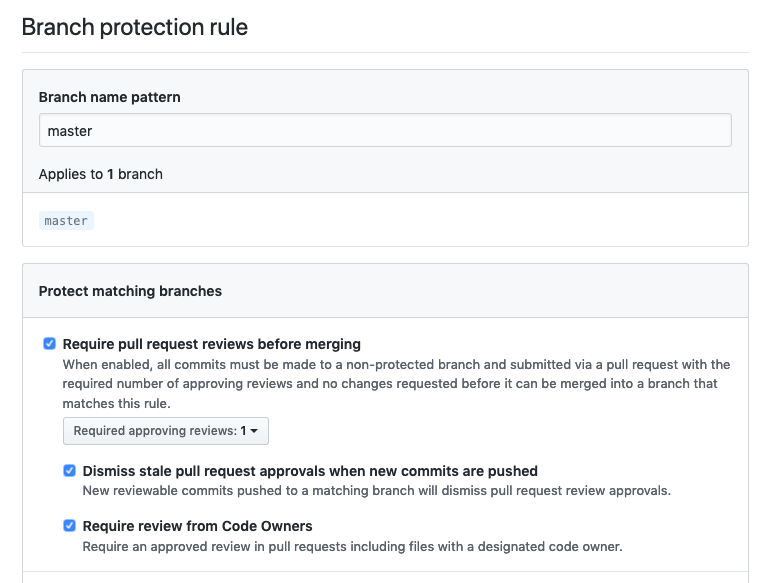
\includegraphics[scale=0.50]{images/github-branch-protection.png}
\caption{Setting up branch protection.}
\label{branchprotect}
\end{figure}

\justify{}
After we start to work with CI/CD tools (status checks, like GitHub Actions for example) new choices, as seen in figure \ref{statuscheck}, become
available in this part of your repository for managing those checks.

\begin{figure}
\centering
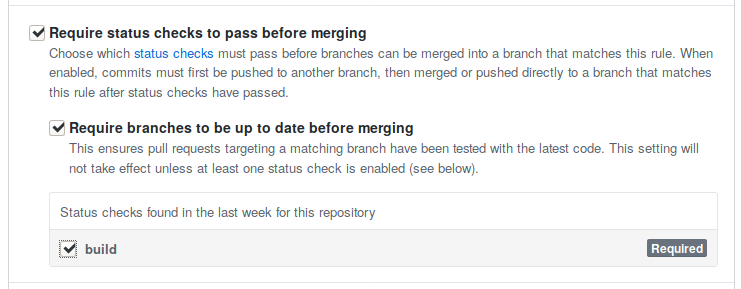
\includegraphics[scale=0.53]{images/guthub-status-check.png}
\caption{Requiring status checks.}
\label{statuscheck}
\end{figure}

\section{Branching and Merging}
\subsection{Working with Branches}

\justify{}
Naming your branches something useful is helpful (self documenting). Let's look at how to create a branch.

\subsection{Pull Requests}

\justify{}
When you make changes on a local branch, say on your personal laptop, you will eventually want those changes
to flow back into the main project. Opening a pull request\index{Pull Request} is a means of letting other
people know you've got a set of changes ready for review and potential changes.

\justify{}
Keeping pull requests smaller and more frequent makes it easier for your
peers to review your changes. It also means you will be less likely to lose work.

\subsection{Merging Your Branch}

\markdownInput{../labs/ch5/lab-5b.md}

\section{Forking and Cloning Existing Repositories}

\justify{}
When someone else has a project on github.com that you would like to make changes to, you can make a ``fork'' of that project.
Forking\index{forking} a repository means you are making a copy of that repository to your personal account on the GitHub web
site. The reason for creating a fork is so we can make and test changes without any impact on the original repository.

\justify{}
Once you have created a fork, you create a locay copy of your fork on one or more of your personal workstations. This is
known as creating a ``clone''\index{cloning a repo} of your fork. Now we have a workspace to make and test changes without
any impact to the parent repository. These changes or completed by creating one or more ``branches''. These branches and the
changes they encompass can be tested further, and are eventually merged into the parent repository.

\begin{figure}[!htb]
\centering

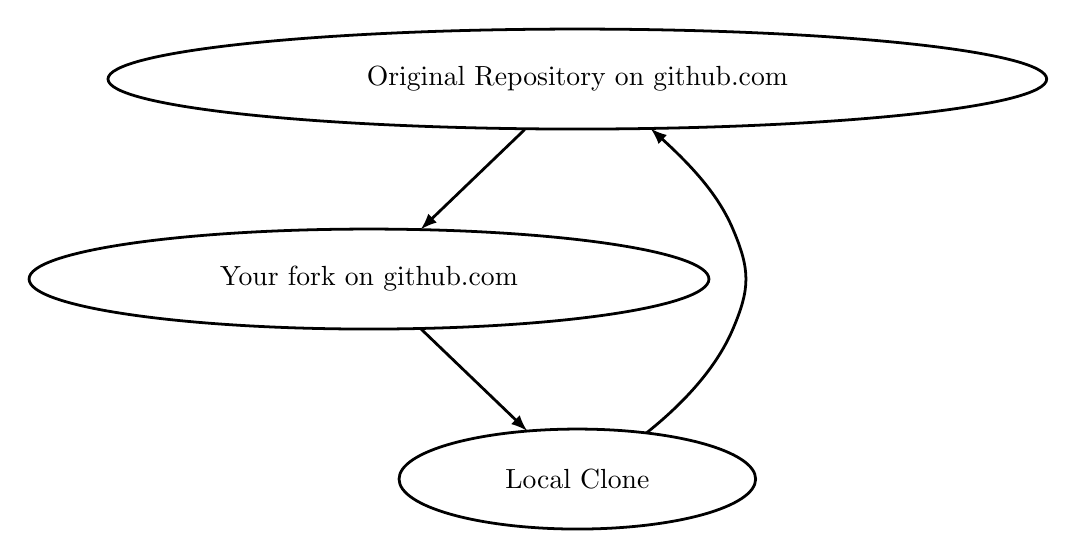
\begin{tikzpicture}[>=latex,line join=bevel,]
  \pgfsetlinewidth{1bp}
%%
\pgfsetcolor{black}
  % Edge: orig -> fork
  \draw [->] (178.26bp,143.83bp) .. controls (169.13bp,135.07bp) and (158.04bp,124.42bp)  .. (140.85bp,107.91bp);
  % Edge: fork -> clone
  \draw [->] (140.73bp,72.202bp) .. controls (150.06bp,63.242bp) and (161.52bp,52.241bp)  .. (179.12bp,35.345bp);
  % Edge: clone -> orig
  \draw [->] (222.15bp,34.664bp) .. controls (233.94bp,44.073bp) and (246.8bp,56.959bp)  .. (253.19bp,72.0bp) .. controls (259.45bp,86.726bp) and (259.45bp,93.274bp)  .. (253.19bp,108.0bp) .. controls (248.45bp,119.15bp) and (240.16bp,129.12bp)  .. (223.62bp,144.15bp);
  % Node: orig
\begin{scope}
  \definecolor{strokecol}{rgb}{0.0,0.0,0.0};
  \pgfsetstrokecolor{strokecol}
  \draw (197.19bp,162.0bp) ellipse (168.97bp and 18.0bp);
  \draw (197.19bp,162.0bp) node {Original Repository on github.com};
\end{scope}
  % Node: fork
\begin{scope}
  \definecolor{strokecol}{rgb}{0.0,0.0,0.0};
  \pgfsetstrokecolor{strokecol}
  \draw (122.19bp,90.0bp) ellipse (122.38bp and 18.0bp);
  \draw (122.19bp,90.0bp) node {Your fork on github.com};
\end{scope}
  % Node: clone
\begin{scope}
  \definecolor{strokecol}{rgb}{0.0,0.0,0.0};
  \pgfsetstrokecolor{strokecol}
  \draw (197.19bp,18.0bp) ellipse (64.19bp and 18.0bp);
  \draw (197.19bp,18.0bp) node {Local Clone};
\end{scope}
%
\end{tikzpicture}


\caption{Forking and cloning.}
\label{forkandclone}
\end{figure}

\justify{}
This can be a tricky pattern to master, but it is fundamental if you
want to join the ranks of Open Source contributors and developers that
enjoy the full power of Git and GitHub.

\justify{}
Adding a ``remote'' to your repository clone is a git convention to easily manage branches between your clone and
the original source repository.

\justify{}
If you are starting out on a new project, simply creating a repo is probably enough. The whole fork/clone/merge to original
paradigm is better suited to medium to large size projects that accept contributions from multiple developers.

\markdownInput{../labs/ch5/lab-5c.md}

\section{Template Repositories}

\justify{}
A GitHub Template Repository is available should you decide to follow along with the code examples in this book. The next sets of steps are
predicated on having Docker installed and running as described in the previous chapter.

\markdownInput{../labs/ch5/lab-5d.md}

\section{Conventions}

\subsection{CODEOWNERS}

\justify{}
Creating a CODEOWNERS\index{CODEOWNERS} file is a good way to automatically tag folks in PRs to make them aware of
changes to certain files or folders in your projects.

\justify{}
In it's most basic form, the CODEOWNERS file in the .github directory
simply lists the file(s) and the owner(s) on a line together.

\justify{}
Consider this example where we add the @hotpeppersec to the CODEOWNERS file.

\begin{mybox}{\thetcbcounter: Adding a user to CODEOWNERS file}
      \lstinputlisting{code/22-github/create-codeowners.txt}
\end{mybox}

\justify{}
In this example, the @githubusername user will be tagged as a reviewer in all pull requests.

\subsection{The .gitignore file}

\justify{}
Use this file\index{.gitignore} to designate items that should be excluded from revision
control. This is useful for helping keep credentials and other secrets out of the GitHub repository.

\justify{}
Consider the following example .gitignore file. This will prevent you from checking in the .DS-Store that
Macintosh creates in many folders.

\begin{mybox}{\thetcbcounter: Example .gitignore file}
      \lstinputlisting{code/22-github/create-gitignore.txt}
\end{mybox}

\section{Automated Repository Scanning}

\justify{}
There are many GitHub plugins that are free for single-user/non-commercial scenarios. a cursory search of the web of the
GitHub Marketplace will turn up many of these. Let's leave some of the
tedious work to the bots, allowing us to focus on our DevSecOps journey to the cloud!

\justify{}
\begin{tabular}{| p{2.3cm}| p{4.5cm} | p{8.5cm} |}
      \hline
      \textbf{Tool}& \textbf{Purpose}& \textbf{Source} \\
      \hline
      Renovate & dependency scanner & web site \\
      \hline
      lgtm & puppet-lint & Looks Good To Me \url{http://puppet-lint.com/} \\
      \hline
      metabob & AI based code review tool & python (pip install pylint/flake8) \\
      \hline
      bridgecrew & PR security scanner & web site \\
      \hline
\end{tabular}

\section{Further Reading}

\clearpage

\section{Directory Structure}

\justify{}
Relevant files and folders mentioned in this chapter are organized as
seen below.

\begin{figure}[!htb]
      \centering
      \chapter{Revision Control}

\includegraphics[scale=0.20]{images/owl-50267_1920.jpg}

\justifying
Using a revision control\index{revision control} methodology allows us to organize and store project artifacts. Typically these
artifacts are source code files but may include documentation, files to assist us with Kubernetes cluster management and application
deployment, and more. Websites like \href{https://github.com}{github.com} for example, are the modern
backbone of revision control, and foundational to our workflow. They are a key piece of our software delivery pipeline,
allowing us to declare a single source of truth for the code that makes up our project. Multiple users or teams can collaborate on a
single code base stored in a repository, the structure which encompasses a typical project. Even after the benefits from collaboration and
storage are considered, we can still realize a great benefit from being able to create releases, which can be tagged and ``rolled''
forward to and back from.

\justifying
There are other similar services we can choose from. These tend to be free for personal projects, non-commercial, and even some commercial
uses. For example \href{https://bitbucket.org/product}{Bitbucket} and \href{https://about.gitlab.com/}{GitLab}. For the purposes of this
book we will focus GitHub\index{GitHub}, since many people are familiar with it.

\justifying
Git is the tool that allows for revision control of your work. GitHub is a repository for storing that work, creating
teams to work on projects, tracking issues, defining release packages, and more. Simply put, \href{github.com}{github.com}
is a website that gives you a place to store the work you are using git to manage. Git was created in 2005 by
Linus Torvalds\index{Linus Torvalds}, who, as you may know, also created the Linux kernel.

\justifying
After creating your account on GitHub, one of the very first things you should do is to configure two-factor authentication (2FA)\index{2FA} for your GitHub account.
See \href{https://docs.github.com/en/github/authenticating-to-github/securing-your-account-with-two-factor-authentication-2fa}{securing your account with two factor authentication}
for more information. If you already have an account at GitHub, now is a good time to make sure you have this feature enabled. Two-factor authentication provides
an additional layer of security on your Github account, and is all-around good practice. Using two- or multi-factor authentication with a
password manager will do wonders
to improve your security hygiene. You may also use your password manager to store your account recovery codes. Creating a text file
that contains your recovery codes and keeping an encrypted copy in your home directory is another option.

\section{Creating a Repository}

Repository creation is well documented, for example
\href{https://docs.github.com/en/get-started/quickstart/create-a-repo}{these steps in the GitHub quick start pages}. Let look a bit
more closely ar what is involved in this process.

\justifying
Often I will start a new repository on my personal account while I use the steps in this book to get the project off the ground.
Later I will move the repository into an organization where the responsibility for ownership and administration can be
shared with other folks.

\justifying
Directions for the labs in this chapter are located in GitHub, of course!
\href{https://github.com/devsecfranklin/devsecops-tactical-workbook/tree/main/code/ch5}{Follow this link to view the lab files},
or simply proceed with the steps below.

\justifying
So far we have created the files seen in figure \ref{projfiles} to our project. There is much to be gained from bringing our project under revision control so let's
make that our next task. Take note, the ``top level'' for our GitHub repository will be the ``myproject'' folder even though we have some files in our ``/home/devsecops''
home directory that impact our project. We want to keep a separation between the source code and documentation in the ``myproject'' folder and any machine specific
configuration that is present on an individual developers workstation.

\begin{figure}[!htb]
\centering

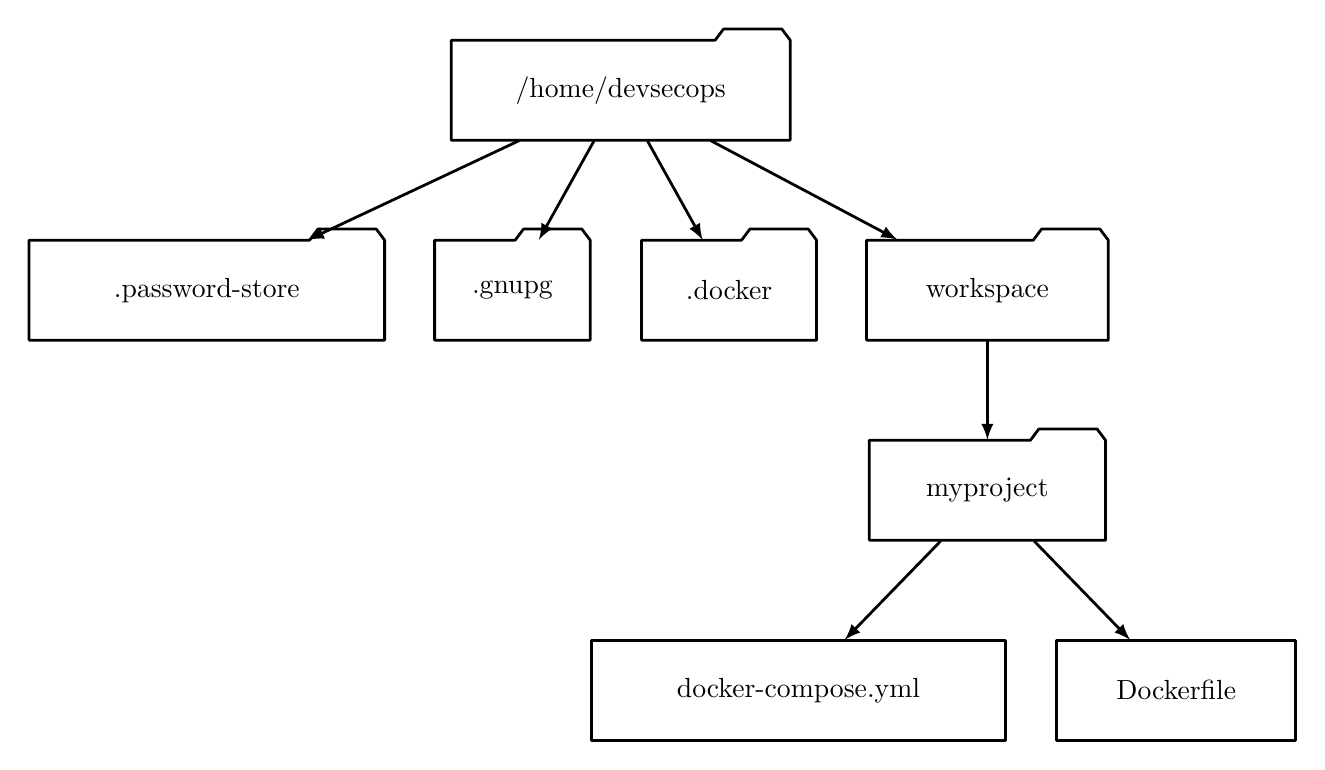
\begin{tikzpicture}[>=latex,line join=bevel,]
  \pgfsetlinewidth{1bp}
%%
\pgfsetcolor{black}
  % Edge: framework -> pass
  \draw [->] (176.55bp,215.88bp) .. controls (156.36bp,206.39bp) and (131.08bp,194.51bp)  .. (100.33bp,180.07bp);
  % Edge: framework -> gnupg
  \draw [->] (203.36bp,215.7bp) .. controls (198.87bp,207.64bp) and (193.44bp,197.89bp)  .. (183.53bp,180.1bp);
  % Edge: framework -> docker
  \draw [->] (222.64bp,215.7bp) .. controls (227.13bp,207.64bp) and (232.56bp,197.89bp)  .. (242.47bp,180.1bp);
  % Edge: framework -> workspace
  \draw [->] (245.29bp,215.88bp) .. controls (262.87bp,206.55bp) and (284.81bp,194.92bp)  .. (312.59bp,180.19bp);
  % Edge: workspace -> myproject
  \draw [->] (345.0bp,143.7bp) .. controls (345.0bp,135.98bp) and (345.0bp,126.71bp)  .. (345.0bp,108.1bp);
  % Edge: myproject -> dockercom
  \draw [->] (328.19bp,71.697bp) .. controls (319.87bp,63.135bp) and (309.69bp,52.656bp)  .. (293.62bp,36.104bp);
  % Edge: myproject -> Dockerfile
  \draw [->] (361.81bp,71.697bp) .. controls (370.13bp,63.135bp) and (380.31bp,52.656bp)  .. (396.38bp,36.104bp);
  % Node: framework
\begin{scope}
  \definecolor{strokecol}{rgb}{0.0,0.0,0.0};
  \pgfsetstrokecolor{strokecol}
  \draw (274.0bp,252.0bp) -- (271.0bp,256.0bp) -- (250.0bp,256.0bp) -- (247.0bp,252.0bp) -- (152.0bp,252.0bp) -- (152.0bp,216.0bp) -- (274.0bp,216.0bp) -- cycle;
  \draw (213.0bp,234.0bp) node {/home/devsecops};
\end{scope}
  % Node: pass
\begin{scope}
  \definecolor{strokecol}{rgb}{0.0,0.0,0.0};
  \pgfsetstrokecolor{strokecol}
  \draw (128.0bp,180.0bp) -- (125.0bp,184.0bp) -- (104.0bp,184.0bp) -- (101.0bp,180.0bp) -- (0.0bp,180.0bp) -- (0.0bp,144.0bp) -- (128.0bp,144.0bp) -- cycle;
  \draw (64.0bp,162.0bp) node {.password-store};
\end{scope}
  % Node: gnupg
\begin{scope}
  \definecolor{strokecol}{rgb}{0.0,0.0,0.0};
  \pgfsetstrokecolor{strokecol}
  \draw (202.0bp,180.0bp) -- (199.0bp,184.0bp) -- (178.0bp,184.0bp) -- (175.0bp,180.0bp) -- (146.0bp,180.0bp) -- (146.0bp,144.0bp) -- (202.0bp,144.0bp) -- cycle;
  \draw (174.0bp,162.0bp) node {.gnupg};
\end{scope}
  % Node: docker
\begin{scope}
  \definecolor{strokecol}{rgb}{0.0,0.0,0.0};
  \pgfsetstrokecolor{strokecol}
  \draw (283.5bp,180.0bp) -- (280.5bp,184.0bp) -- (259.5bp,184.0bp) -- (256.5bp,180.0bp) -- (220.5bp,180.0bp) -- (220.5bp,144.0bp) -- (283.5bp,144.0bp) -- cycle;
  \draw (252.0bp,162.0bp) node {.docker};
\end{scope}
  % Node: workspace
\begin{scope}
  \definecolor{strokecol}{rgb}{0.0,0.0,0.0};
  \pgfsetstrokecolor{strokecol}
  \draw (388.5bp,180.0bp) -- (385.5bp,184.0bp) -- (364.5bp,184.0bp) -- (361.5bp,180.0bp) -- (301.5bp,180.0bp) -- (301.5bp,144.0bp) -- (388.5bp,144.0bp) -- cycle;
  \draw (345.0bp,162.0bp) node {workspace};
\end{scope}
  % Node: myproject
\begin{scope}
  \definecolor{strokecol}{rgb}{0.0,0.0,0.0};
  \pgfsetstrokecolor{strokecol}
  \draw (387.5bp,108.0bp) -- (384.5bp,112.0bp) -- (363.5bp,112.0bp) -- (360.5bp,108.0bp) -- (302.5bp,108.0bp) -- (302.5bp,72.0bp) -- (387.5bp,72.0bp) -- cycle;
  \draw (345.0bp,90.0bp) node {myproject};
\end{scope}
  % Node: dockercom
\begin{scope}
  \definecolor{strokecol}{rgb}{0.0,0.0,0.0};
  \pgfsetstrokecolor{strokecol}
  \draw (351.5bp,36.0bp) -- (202.5bp,36.0bp) -- (202.5bp,0.0bp) -- (351.5bp,0.0bp) -- cycle;
  \draw (277.0bp,18.0bp) node {docker-compose.yml};
\end{scope}
  % Node: Dockerfile
\begin{scope}
  \definecolor{strokecol}{rgb}{0.0,0.0,0.0};
  \pgfsetstrokecolor{strokecol}
  \draw (456.0bp,36.0bp) -- (370.0bp,36.0bp) -- (370.0bp,0.0bp) -- (456.0bp,0.0bp) -- cycle;
  \draw (413.0bp,18.0bp) node {Dockerfile};
\end{scope}
%
\end{tikzpicture}


\caption{Project files.}
\label{projfiles}
\end{figure}

\markdownInput{../labs/ch5/lab-5a.md}

\subsection{Repository Settings}

\justifying
When setting up a new repository in my GitHub account, I always click the Settings tab (with the little gear icon) and then choose the
``Branches'' section. The Default branch gets set to ``main''. Clicking the ``Add Rule'' button, entering ``main'' for the ``Branch name pattern'',
and then the green ``Create'' button sets up master as a protected branch. Consider the following example \ref{branchprotect}.

\begin{figure}[!htb]
\centering
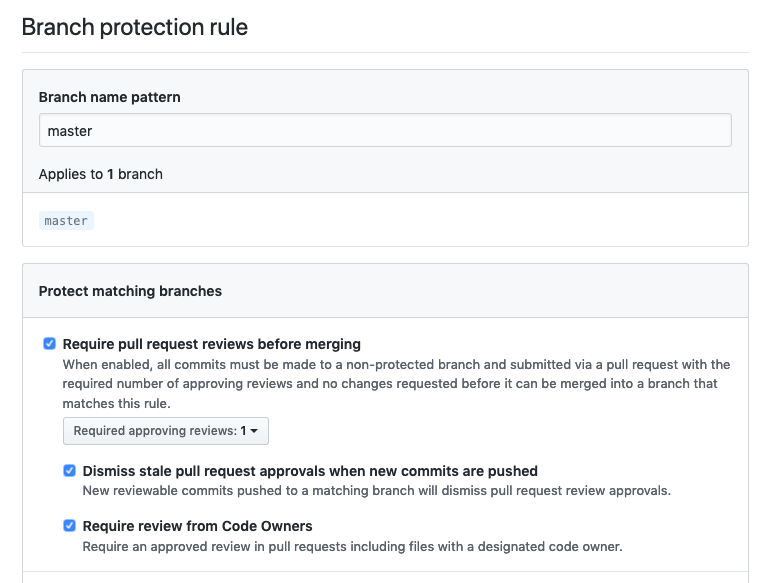
\includegraphics[scale=0.50]{images/github-branch-protection.png}
\caption{Setting up branch protection.}
\label{branchprotect}
\end{figure}

\justifying
After we start to work with CI/CD tools (status checks, like GitHub Actions for example) new choices, as seen in figure \ref{statuscheck}, become
available in this part of your repository for managing those checks.

\begin{figure}
\centering
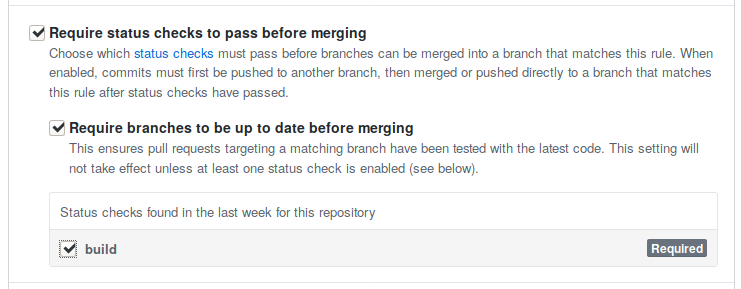
\includegraphics[scale=0.53]{images/guthub-status-check.png}
\caption{Requiring status checks.}
\label{statuscheck}
\end{figure}

\section{Branching and Merging}

When we say we are going to create a branch with git, it simply means we are going to take a snapshot of the code base at a point in time, and make our changes on that snapshot. The goal is to be able to make fixes and improvements without impacting the original code base.
Once our changes are completed, the typical process is to request a review from other team members and do some testing to make sure the changes will perform as expected. Once this is done, we are ready to merge our updated branch back into the main code base.

\subsection{Working with Branches}

\justifying
Naming your branches something useful is helpful (self documenting). Let's look at how to create a branch.

\subsection{Pull Requests}

\justifying
When you make changes on a local branch, say on your personal laptop, you will eventually want those changes
to flow back into the main project. Opening a pull request\index{Pull Request} is a means of letting other
people know you've got a set of changes ready for review and potential changes.

\justifying
Keeping pull requests smaller and more frequent makes it easier for your
peers to review your changes. It also means you will be less likely to lose work.

\subsection{Merging Your Branch}

\markdownInput{../labs/ch5/lab-5b.md}

\section{Forking and Cloning Existing Repositories}

\justifying
When someone else has a project on github.com that you would like to make changes to, you can make a ``fork'' of that project.
Forking\index{forking} a repository means you are making a copy of that repository to your personal account on the GitHub web
site. The reason for creating a fork is so we can make and test changes without any impact on the original repository.

\justifying
Once you have created a fork, you create a local copy of your fork on one or more of your personal workstations. This is
known as creating a ``clone'' \index{cloning a repo} of your fork. Now we have a workspace to make and test changes without
any impact to the parent repository. These changes or completed by creating one or more ``branches''. These branches and the
changes they encompass can be tested further, and are eventually merged into the parent repository.

\begin{figure}[!htb]
\centering

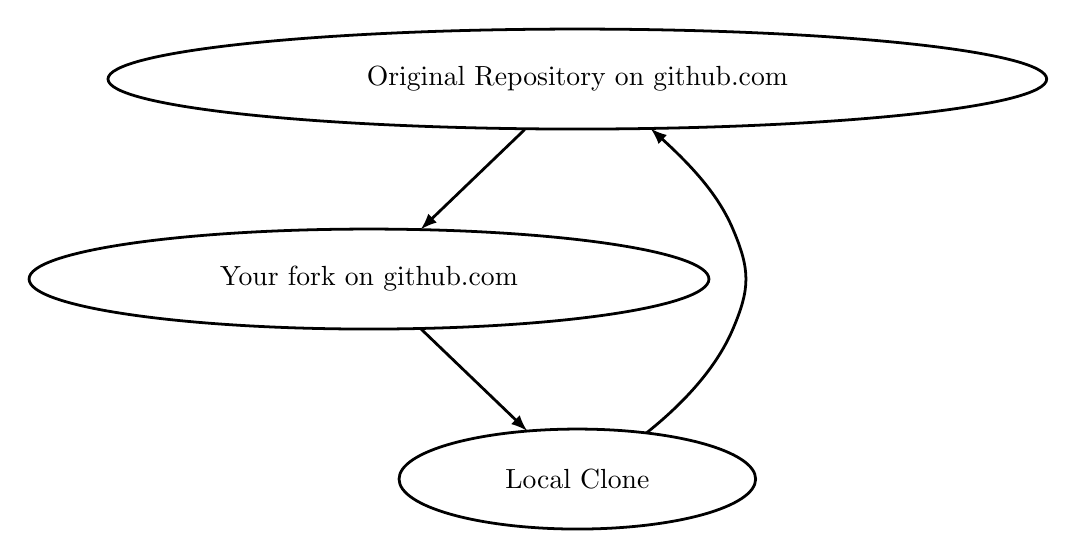
\begin{tikzpicture}[>=latex,line join=bevel,]
  \pgfsetlinewidth{1bp}
%%
\pgfsetcolor{black}
  % Edge: orig -> fork
  \draw [->] (178.26bp,143.83bp) .. controls (169.13bp,135.07bp) and (158.04bp,124.42bp)  .. (140.85bp,107.91bp);
  % Edge: fork -> clone
  \draw [->] (140.73bp,72.202bp) .. controls (150.06bp,63.242bp) and (161.52bp,52.241bp)  .. (179.12bp,35.345bp);
  % Edge: clone -> orig
  \draw [->] (222.15bp,34.664bp) .. controls (233.94bp,44.073bp) and (246.8bp,56.959bp)  .. (253.19bp,72.0bp) .. controls (259.45bp,86.726bp) and (259.45bp,93.274bp)  .. (253.19bp,108.0bp) .. controls (248.45bp,119.15bp) and (240.16bp,129.12bp)  .. (223.62bp,144.15bp);
  % Node: orig
\begin{scope}
  \definecolor{strokecol}{rgb}{0.0,0.0,0.0};
  \pgfsetstrokecolor{strokecol}
  \draw (197.19bp,162.0bp) ellipse (168.97bp and 18.0bp);
  \draw (197.19bp,162.0bp) node {Original Repository on github.com};
\end{scope}
  % Node: fork
\begin{scope}
  \definecolor{strokecol}{rgb}{0.0,0.0,0.0};
  \pgfsetstrokecolor{strokecol}
  \draw (122.19bp,90.0bp) ellipse (122.38bp and 18.0bp);
  \draw (122.19bp,90.0bp) node {Your fork on github.com};
\end{scope}
  % Node: clone
\begin{scope}
  \definecolor{strokecol}{rgb}{0.0,0.0,0.0};
  \pgfsetstrokecolor{strokecol}
  \draw (197.19bp,18.0bp) ellipse (64.19bp and 18.0bp);
  \draw (197.19bp,18.0bp) node {Local Clone};
\end{scope}
%
\end{tikzpicture}


\caption{Forking and cloning.}
\label{forkandclone}
\end{figure}

\justifying
This can be a tricky pattern to master, but it is fundamental if you
want to join the ranks of Open Source contributors and developers that
enjoy the full power of Git and GitHub.

\justifying
Adding a ``remote'' to your repository clone is a git convention to easily manage branches between your clone and
the original source repository.

\justifying
If you are starting out on a new project, simply creating a repo is probably enough. The whole fork/clone/merge to original
paradigm is better suited to medium to large size projects that accept contributions from multiple developers.

\markdownInput{../labs/ch5/lab-5c.md}

\section{Template Repositories}

\justifying
A GitHub Template Repository is available should you decide to follow along with the code examples in this book. The next sets of steps are
predicated on having Docker installed and running as described in the previous chapter.

\markdownInput{../labs/ch5/lab-5d.md}

\section{Conventions}

\subsection{CODEOWNERS}

\justifying
Creating a CODEOWNERS\index{CODEOWNERS} file is a good way to automatically tag folks in pull requests to make them aware of
changes to certain files or folders in your projects.

\justifying
In it's most basic form, the CODEOWNERS file in the .github directory simply lists the file(s) and the owner(s) on a line together.

\justifying
Consider this example where we add the ``@kevinflynn'' user to the CODEOWNERS file.

\begin{mybox}{\thetcbcounter: Adding a user to CODEOWNERS file}
      \lstinputlisting{code/22-github/create-codeowners.txt}
\end{mybox}

\justifying
In this example, the ``@kevinflynn'' user will be tagged as a reviewer in all pull requests.

\subsection{The .gitignore file}

\justifying
Use this file\index{.gitignore} to designate items that should be excluded from revision
control. This is useful for helping keep credentials and other secrets out of the GitHub repository.

\justifying
Consider the following example .gitignore file. This will prevent you from checking in the .DS-Store that
Macintosh creates in many folders.

\begin{mybox}{\thetcbcounter: Example .gitignore file}
      \lstinputlisting{code/22-github/create-gitignore.txt}
\end{mybox}

\section{Automated Repository Scanning}

\justifying
There are many GitHub plugins that are free for single-user/non-commercial scenarios. a cursory search of the web of the
GitHub Marketplace will turn up many of these. Let's leave some of the
tedious work to the bots, allowing us to focus on our DevSecOps journey to the cloud!

\justifying
\begin{tabular}{| p{2.3cm}| p{4.5cm} | p{8.5cm} |}
      \hline
     \textbf{Tool}& \textbf{Purpose}& \textbf{Source} \\
      \hline
      Renovate & dependency scanner & web site \\
      \hline
      lgtm & puppet-lint & Looks Good To Me \url{http://puppet-lint.com/} \\
      \hline
      metabob & AI based code review tool & website \\
      \hline
      bridgecrew & PR security scanner & web site \\
      \hline
\end{tabular}

\section{Directory Structure}

\justifying
Relevant files and folders mentioned in this chapter are organized as seen below.

\begin{figure}[!htb]
      \centering
      \chapter{Revision Control}

\includegraphics[scale=0.20]{images/owl-50267_1920.jpg}

\justifying
Using a revision control\index{revision control} methodology allows us to organize and store project artifacts. Typically these
artifacts are source code files but may include documentation, files to assist us with Kubernetes cluster management and application
deployment, and more. Websites like \href{https://github.com}{github.com} for example, are the modern
backbone of revision control, and foundational to our workflow. They are a key piece of our software delivery pipeline,
allowing us to declare a single source of truth for the code that makes up our project. Multiple users or teams can collaborate on a
single code base stored in a repository, the structure which encompasses a typical project. Even after the benefits from collaboration and
storage are considered, we can still realize a great benefit from being able to create releases, which can be tagged and ``rolled''
forward to and back from.

\justifying
There are other similar services we can choose from. These tend to be free for personal projects, non-commercial, and even some commercial
uses. For example \href{https://bitbucket.org/product}{Bitbucket} and \href{https://about.gitlab.com/}{GitLab}. For the purposes of this
book we will focus GitHub\index{GitHub}, since many people are familiar with it.

\justifying
Git is the tool that allows for revision control of your work. GitHub is a repository for storing that work, creating
teams to work on projects, tracking issues, defining release packages, and more. Simply put, \href{github.com}{github.com}
is a website that gives you a place to store the work you are using git to manage. Git was created in 2005 by
Linus Torvalds\index{Linus Torvalds}, who, as you may know, also created the Linux kernel.

\justifying
After creating your account on GitHub, one of the very first things you should do is to configure two-factor authentication (2FA)\index{2FA} for your GitHub account.
See \href{https://docs.github.com/en/github/authenticating-to-github/securing-your-account-with-two-factor-authentication-2fa}{securing your account with two factor authentication}
for more information. If you already have an account at GitHub, now is a good time to make sure you have this feature enabled. Two-factor authentication provides
an additional layer of security on your Github account, and is all-around good practice. Using two- or multi-factor authentication with a
password manager will do wonders
to improve your security hygiene. You may also use your password manager to store your account recovery codes. Creating a text file
that contains your recovery codes and keeping an encrypted copy in your home directory is another option.

\section{Creating a Repository}

Repository creation is well documented, for example
\href{https://docs.github.com/en/get-started/quickstart/create-a-repo}{these steps in the GitHub quick start pages}. Let look a bit
more closely ar what is involved in this process.

\justifying
Often I will start a new repository on my personal account while I use the steps in this book to get the project off the ground.
Later I will move the repository into an organization where the responsibility for ownership and administration can be
shared with other folks.

\justifying
Directions for the labs in this chapter are located in GitHub, of course!
\href{https://github.com/devsecfranklin/devsecops-tactical-workbook/tree/main/code/ch5}{Follow this link to view the lab files},
or simply proceed with the steps below.

\justifying
So far we have created the files seen in figure \ref{projfiles} to our project. There is much to be gained from bringing our project under revision control so let's
make that our next task. Take note, the ``top level'' for our GitHub repository will be the ``myproject'' folder even though we have some files in our ``/home/devsecops''
home directory that impact our project. We want to keep a separation between the source code and documentation in the ``myproject'' folder and any machine specific
configuration that is present on an individual developers workstation.

\begin{figure}[!htb]
\centering

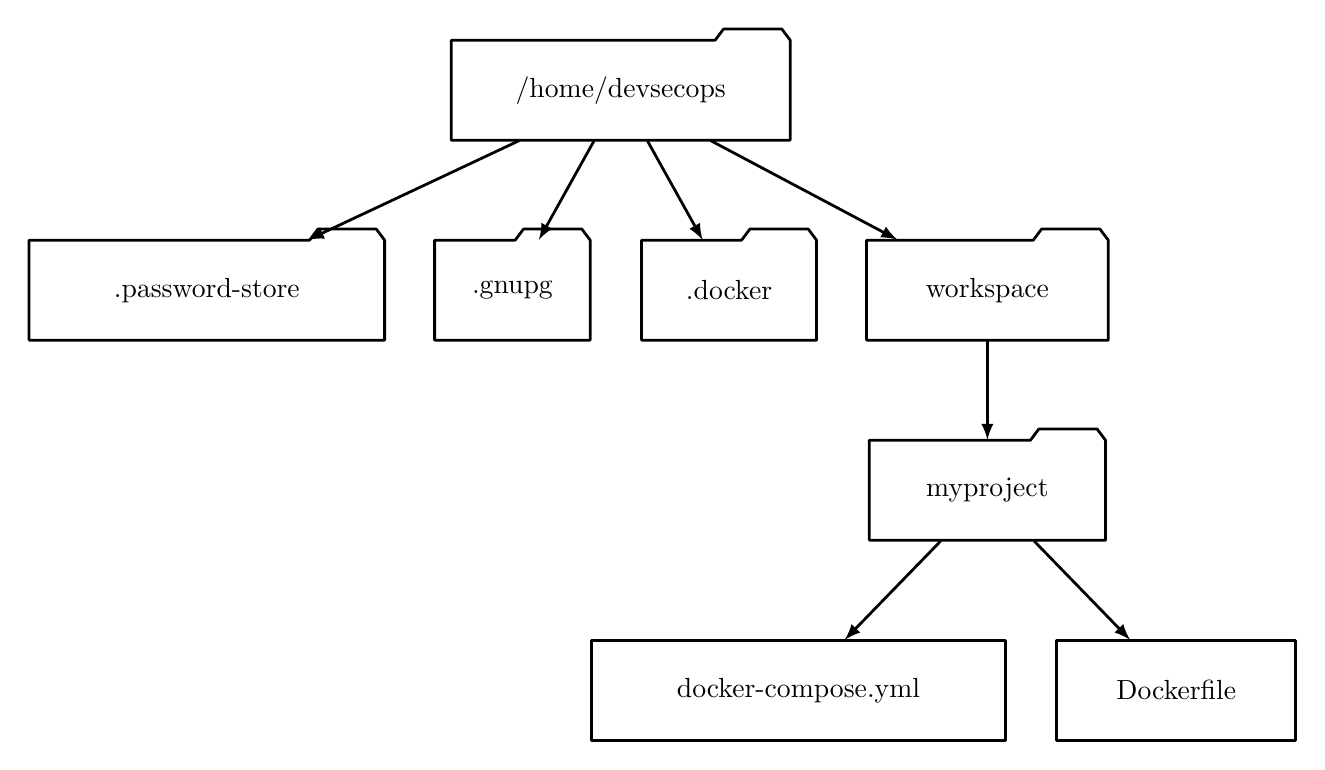
\begin{tikzpicture}[>=latex,line join=bevel,]
  \pgfsetlinewidth{1bp}
%%
\pgfsetcolor{black}
  % Edge: framework -> pass
  \draw [->] (176.55bp,215.88bp) .. controls (156.36bp,206.39bp) and (131.08bp,194.51bp)  .. (100.33bp,180.07bp);
  % Edge: framework -> gnupg
  \draw [->] (203.36bp,215.7bp) .. controls (198.87bp,207.64bp) and (193.44bp,197.89bp)  .. (183.53bp,180.1bp);
  % Edge: framework -> docker
  \draw [->] (222.64bp,215.7bp) .. controls (227.13bp,207.64bp) and (232.56bp,197.89bp)  .. (242.47bp,180.1bp);
  % Edge: framework -> workspace
  \draw [->] (245.29bp,215.88bp) .. controls (262.87bp,206.55bp) and (284.81bp,194.92bp)  .. (312.59bp,180.19bp);
  % Edge: workspace -> myproject
  \draw [->] (345.0bp,143.7bp) .. controls (345.0bp,135.98bp) and (345.0bp,126.71bp)  .. (345.0bp,108.1bp);
  % Edge: myproject -> dockercom
  \draw [->] (328.19bp,71.697bp) .. controls (319.87bp,63.135bp) and (309.69bp,52.656bp)  .. (293.62bp,36.104bp);
  % Edge: myproject -> Dockerfile
  \draw [->] (361.81bp,71.697bp) .. controls (370.13bp,63.135bp) and (380.31bp,52.656bp)  .. (396.38bp,36.104bp);
  % Node: framework
\begin{scope}
  \definecolor{strokecol}{rgb}{0.0,0.0,0.0};
  \pgfsetstrokecolor{strokecol}
  \draw (274.0bp,252.0bp) -- (271.0bp,256.0bp) -- (250.0bp,256.0bp) -- (247.0bp,252.0bp) -- (152.0bp,252.0bp) -- (152.0bp,216.0bp) -- (274.0bp,216.0bp) -- cycle;
  \draw (213.0bp,234.0bp) node {/home/devsecops};
\end{scope}
  % Node: pass
\begin{scope}
  \definecolor{strokecol}{rgb}{0.0,0.0,0.0};
  \pgfsetstrokecolor{strokecol}
  \draw (128.0bp,180.0bp) -- (125.0bp,184.0bp) -- (104.0bp,184.0bp) -- (101.0bp,180.0bp) -- (0.0bp,180.0bp) -- (0.0bp,144.0bp) -- (128.0bp,144.0bp) -- cycle;
  \draw (64.0bp,162.0bp) node {.password-store};
\end{scope}
  % Node: gnupg
\begin{scope}
  \definecolor{strokecol}{rgb}{0.0,0.0,0.0};
  \pgfsetstrokecolor{strokecol}
  \draw (202.0bp,180.0bp) -- (199.0bp,184.0bp) -- (178.0bp,184.0bp) -- (175.0bp,180.0bp) -- (146.0bp,180.0bp) -- (146.0bp,144.0bp) -- (202.0bp,144.0bp) -- cycle;
  \draw (174.0bp,162.0bp) node {.gnupg};
\end{scope}
  % Node: docker
\begin{scope}
  \definecolor{strokecol}{rgb}{0.0,0.0,0.0};
  \pgfsetstrokecolor{strokecol}
  \draw (283.5bp,180.0bp) -- (280.5bp,184.0bp) -- (259.5bp,184.0bp) -- (256.5bp,180.0bp) -- (220.5bp,180.0bp) -- (220.5bp,144.0bp) -- (283.5bp,144.0bp) -- cycle;
  \draw (252.0bp,162.0bp) node {.docker};
\end{scope}
  % Node: workspace
\begin{scope}
  \definecolor{strokecol}{rgb}{0.0,0.0,0.0};
  \pgfsetstrokecolor{strokecol}
  \draw (388.5bp,180.0bp) -- (385.5bp,184.0bp) -- (364.5bp,184.0bp) -- (361.5bp,180.0bp) -- (301.5bp,180.0bp) -- (301.5bp,144.0bp) -- (388.5bp,144.0bp) -- cycle;
  \draw (345.0bp,162.0bp) node {workspace};
\end{scope}
  % Node: myproject
\begin{scope}
  \definecolor{strokecol}{rgb}{0.0,0.0,0.0};
  \pgfsetstrokecolor{strokecol}
  \draw (387.5bp,108.0bp) -- (384.5bp,112.0bp) -- (363.5bp,112.0bp) -- (360.5bp,108.0bp) -- (302.5bp,108.0bp) -- (302.5bp,72.0bp) -- (387.5bp,72.0bp) -- cycle;
  \draw (345.0bp,90.0bp) node {myproject};
\end{scope}
  % Node: dockercom
\begin{scope}
  \definecolor{strokecol}{rgb}{0.0,0.0,0.0};
  \pgfsetstrokecolor{strokecol}
  \draw (351.5bp,36.0bp) -- (202.5bp,36.0bp) -- (202.5bp,0.0bp) -- (351.5bp,0.0bp) -- cycle;
  \draw (277.0bp,18.0bp) node {docker-compose.yml};
\end{scope}
  % Node: Dockerfile
\begin{scope}
  \definecolor{strokecol}{rgb}{0.0,0.0,0.0};
  \pgfsetstrokecolor{strokecol}
  \draw (456.0bp,36.0bp) -- (370.0bp,36.0bp) -- (370.0bp,0.0bp) -- (456.0bp,0.0bp) -- cycle;
  \draw (413.0bp,18.0bp) node {Dockerfile};
\end{scope}
%
\end{tikzpicture}


\caption{Project files.}
\label{projfiles}
\end{figure}

\markdownInput{../labs/ch5/lab-5a.md}

\subsection{Repository Settings}

\justifying
When setting up a new repository in my GitHub account, I always click the Settings tab (with the little gear icon) and then choose the
``Branches'' section. The Default branch gets set to ``main''. Clicking the ``Add Rule'' button, entering ``main'' for the ``Branch name pattern'',
and then the green ``Create'' button sets up master as a protected branch. Consider the following example \ref{branchprotect}.

\begin{figure}[!htb]
\centering
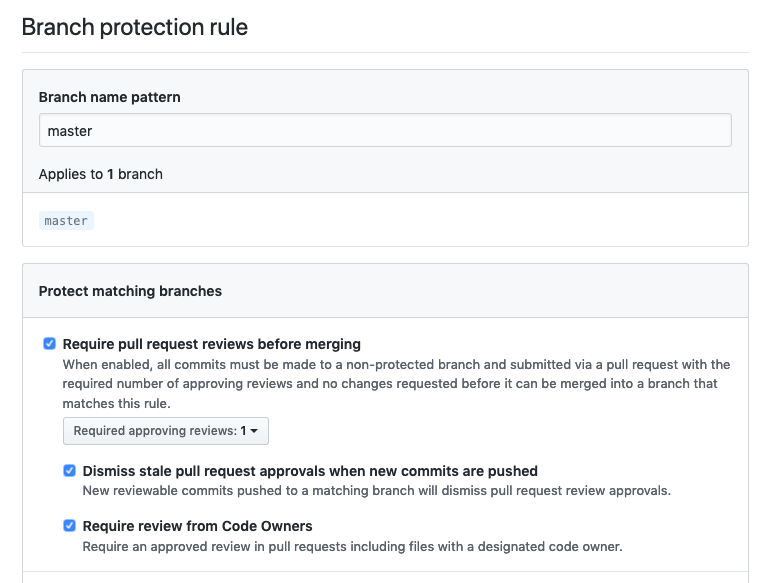
\includegraphics[scale=0.50]{images/github-branch-protection.png}
\caption{Setting up branch protection.}
\label{branchprotect}
\end{figure}

\justifying
After we start to work with CI/CD tools (status checks, like GitHub Actions for example) new choices, as seen in figure \ref{statuscheck}, become
available in this part of your repository for managing those checks.

\begin{figure}
\centering
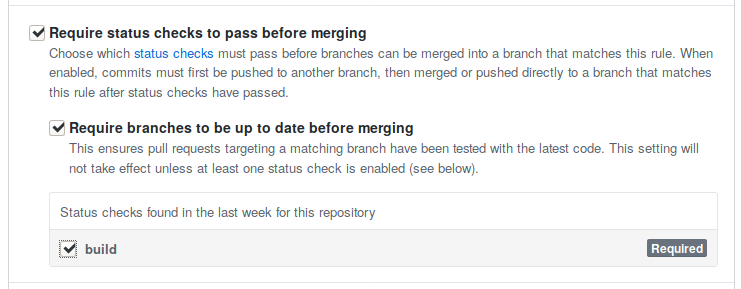
\includegraphics[scale=0.53]{images/guthub-status-check.png}
\caption{Requiring status checks.}
\label{statuscheck}
\end{figure}

\section{Branching and Merging}

When we say we are going to create a branch with git, it simply means we are going to take a snapshot of the code base at a point in time, and make our changes on that snapshot. The goal is to be able to make fixes and improvements without impacting the original code base.
Once our changes are completed, the typical process is to request a review from other team members and do some testing to make sure the changes will perform as expected. Once this is done, we are ready to merge our updated branch back into the main code base.

\subsection{Working with Branches}

\justifying
Naming your branches something useful is helpful (self documenting). Let's look at how to create a branch.

\subsection{Pull Requests}

\justifying
When you make changes on a local branch, say on your personal laptop, you will eventually want those changes
to flow back into the main project. Opening a pull request\index{Pull Request} is a means of letting other
people know you've got a set of changes ready for review and potential changes.

\justifying
Keeping pull requests smaller and more frequent makes it easier for your
peers to review your changes. It also means you will be less likely to lose work.

\subsection{Merging Your Branch}

\markdownInput{../labs/ch5/lab-5b.md}

\section{Forking and Cloning Existing Repositories}

\justifying
When someone else has a project on github.com that you would like to make changes to, you can make a ``fork'' of that project.
Forking\index{forking} a repository means you are making a copy of that repository to your personal account on the GitHub web
site. The reason for creating a fork is so we can make and test changes without any impact on the original repository.

\justifying
Once you have created a fork, you create a local copy of your fork on one or more of your personal workstations. This is
known as creating a ``clone'' \index{cloning a repo} of your fork. Now we have a workspace to make and test changes without
any impact to the parent repository. These changes or completed by creating one or more ``branches''. These branches and the
changes they encompass can be tested further, and are eventually merged into the parent repository.

\begin{figure}[!htb]
\centering

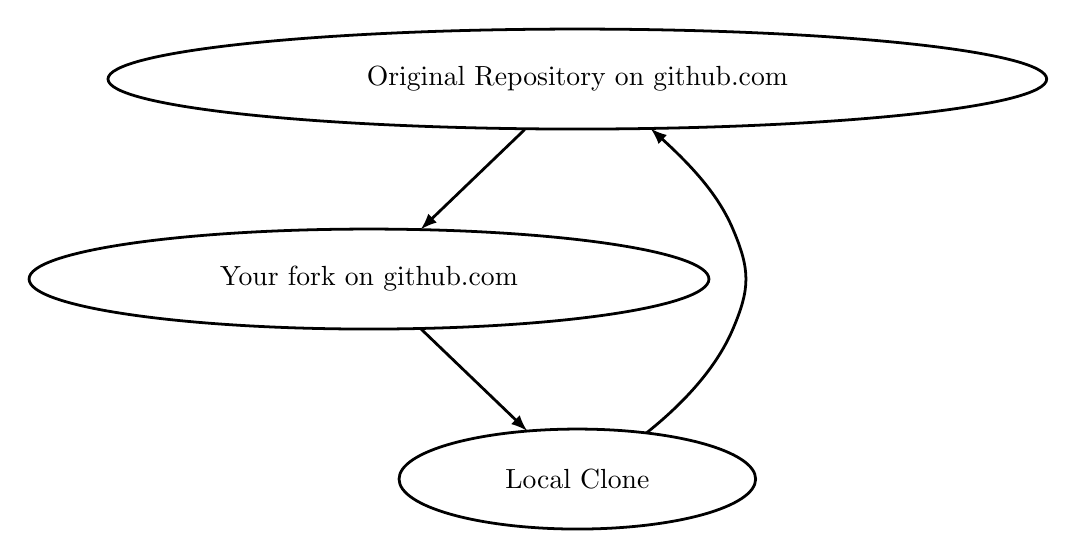
\begin{tikzpicture}[>=latex,line join=bevel,]
  \pgfsetlinewidth{1bp}
%%
\pgfsetcolor{black}
  % Edge: orig -> fork
  \draw [->] (178.26bp,143.83bp) .. controls (169.13bp,135.07bp) and (158.04bp,124.42bp)  .. (140.85bp,107.91bp);
  % Edge: fork -> clone
  \draw [->] (140.73bp,72.202bp) .. controls (150.06bp,63.242bp) and (161.52bp,52.241bp)  .. (179.12bp,35.345bp);
  % Edge: clone -> orig
  \draw [->] (222.15bp,34.664bp) .. controls (233.94bp,44.073bp) and (246.8bp,56.959bp)  .. (253.19bp,72.0bp) .. controls (259.45bp,86.726bp) and (259.45bp,93.274bp)  .. (253.19bp,108.0bp) .. controls (248.45bp,119.15bp) and (240.16bp,129.12bp)  .. (223.62bp,144.15bp);
  % Node: orig
\begin{scope}
  \definecolor{strokecol}{rgb}{0.0,0.0,0.0};
  \pgfsetstrokecolor{strokecol}
  \draw (197.19bp,162.0bp) ellipse (168.97bp and 18.0bp);
  \draw (197.19bp,162.0bp) node {Original Repository on github.com};
\end{scope}
  % Node: fork
\begin{scope}
  \definecolor{strokecol}{rgb}{0.0,0.0,0.0};
  \pgfsetstrokecolor{strokecol}
  \draw (122.19bp,90.0bp) ellipse (122.38bp and 18.0bp);
  \draw (122.19bp,90.0bp) node {Your fork on github.com};
\end{scope}
  % Node: clone
\begin{scope}
  \definecolor{strokecol}{rgb}{0.0,0.0,0.0};
  \pgfsetstrokecolor{strokecol}
  \draw (197.19bp,18.0bp) ellipse (64.19bp and 18.0bp);
  \draw (197.19bp,18.0bp) node {Local Clone};
\end{scope}
%
\end{tikzpicture}


\caption{Forking and cloning.}
\label{forkandclone}
\end{figure}

\justifying
This can be a tricky pattern to master, but it is fundamental if you
want to join the ranks of Open Source contributors and developers that
enjoy the full power of Git and GitHub.

\justifying
Adding a ``remote'' to your repository clone is a git convention to easily manage branches between your clone and
the original source repository.

\justifying
If you are starting out on a new project, simply creating a repo is probably enough. The whole fork/clone/merge to original
paradigm is better suited to medium to large size projects that accept contributions from multiple developers.

\markdownInput{../labs/ch5/lab-5c.md}

\section{Template Repositories}

\justifying
A GitHub Template Repository is available should you decide to follow along with the code examples in this book. The next sets of steps are
predicated on having Docker installed and running as described in the previous chapter.

\markdownInput{../labs/ch5/lab-5d.md}

\section{Conventions}

\subsection{CODEOWNERS}

\justifying
Creating a CODEOWNERS\index{CODEOWNERS} file is a good way to automatically tag folks in pull requests to make them aware of
changes to certain files or folders in your projects.

\justifying
In it's most basic form, the CODEOWNERS file in the .github directory simply lists the file(s) and the owner(s) on a line together.

\justifying
Consider this example where we add the ``@kevinflynn'' user to the CODEOWNERS file.

\begin{mybox}{\thetcbcounter: Adding a user to CODEOWNERS file}
      \lstinputlisting{code/22-github/create-codeowners.txt}
\end{mybox}

\justifying
In this example, the ``@kevinflynn'' user will be tagged as a reviewer in all pull requests.

\subsection{The .gitignore file}

\justifying
Use this file\index{.gitignore} to designate items that should be excluded from revision
control. This is useful for helping keep credentials and other secrets out of the GitHub repository.

\justifying
Consider the following example .gitignore file. This will prevent you from checking in the .DS-Store that
Macintosh creates in many folders.

\begin{mybox}{\thetcbcounter: Example .gitignore file}
      \lstinputlisting{code/22-github/create-gitignore.txt}
\end{mybox}

\section{Automated Repository Scanning}

\justifying
There are many GitHub plugins that are free for single-user/non-commercial scenarios. a cursory search of the web of the
GitHub Marketplace will turn up many of these. Let's leave some of the
tedious work to the bots, allowing us to focus on our DevSecOps journey to the cloud!

\justifying
\begin{tabular}{| p{2.3cm}| p{4.5cm} | p{8.5cm} |}
      \hline
     \textbf{Tool}& \textbf{Purpose}& \textbf{Source} \\
      \hline
      Renovate & dependency scanner & web site \\
      \hline
      lgtm & puppet-lint & Looks Good To Me \url{http://puppet-lint.com/} \\
      \hline
      metabob & AI based code review tool & website \\
      \hline
      bridgecrew & PR security scanner & web site \\
      \hline
\end{tabular}

\section{Directory Structure}

\justifying
Relevant files and folders mentioned in this chapter are organized as seen below.

\begin{figure}[!htb]
      \centering
      \chapter{Revision Control}

\includegraphics[scale=0.20]{images/owl-50267_1920.jpg}

\justifying
Using a revision control\index{revision control} methodology allows us to organize and store project artifacts. Typically these
artifacts are source code files but may include documentation, files to assist us with Kubernetes cluster management and application
deployment, and more. Websites like \href{https://github.com}{github.com} for example, are the modern
backbone of revision control, and foundational to our workflow. They are a key piece of our software delivery pipeline,
allowing us to declare a single source of truth for the code that makes up our project. Multiple users or teams can collaborate on a
single code base stored in a repository, the structure which encompasses a typical project. Even after the benefits from collaboration and
storage are considered, we can still realize a great benefit from being able to create releases, which can be tagged and ``rolled''
forward to and back from.

\justifying
There are other similar services we can choose from. These tend to be free for personal projects, non-commercial, and even some commercial
uses. For example \href{https://bitbucket.org/product}{Bitbucket} and \href{https://about.gitlab.com/}{GitLab}. For the purposes of this
book we will focus GitHub\index{GitHub}, since many people are familiar with it.

\justifying
Git is the tool that allows for revision control of your work. GitHub is a repository for storing that work, creating
teams to work on projects, tracking issues, defining release packages, and more. Simply put, \href{github.com}{github.com}
is a website that gives you a place to store the work you are using git to manage. Git was created in 2005 by
Linus Torvalds\index{Linus Torvalds}, who, as you may know, also created the Linux kernel.

\justifying
After creating your account on GitHub, one of the very first things you should do is to configure two-factor authentication (2FA)\index{2FA} for your GitHub account.
See \href{https://docs.github.com/en/github/authenticating-to-github/securing-your-account-with-two-factor-authentication-2fa}{securing your account with two factor authentication}
for more information. If you already have an account at GitHub, now is a good time to make sure you have this feature enabled. Two-factor authentication provides
an additional layer of security on your Github account, and is all-around good practice. Using two- or multi-factor authentication with a
password manager will do wonders
to improve your security hygiene. You may also use your password manager to store your account recovery codes. Creating a text file
that contains your recovery codes and keeping an encrypted copy in your home directory is another option.

\section{Creating a Repository}

Repository creation is well documented, for example
\href{https://docs.github.com/en/get-started/quickstart/create-a-repo}{these steps in the GitHub quick start pages}. Let look a bit
more closely ar what is involved in this process.

\justifying
Often I will start a new repository on my personal account while I use the steps in this book to get the project off the ground.
Later I will move the repository into an organization where the responsibility for ownership and administration can be
shared with other folks.

\justifying
Directions for the labs in this chapter are located in GitHub, of course!
\href{https://github.com/devsecfranklin/devsecops-tactical-workbook/tree/main/code/ch5}{Follow this link to view the lab files},
or simply proceed with the steps below.

\justifying
So far we have created the files seen in figure \ref{projfiles} to our project. There is much to be gained from bringing our project under revision control so let's
make that our next task. Take note, the ``top level'' for our GitHub repository will be the ``myproject'' folder even though we have some files in our ``/home/devsecops''
home directory that impact our project. We want to keep a separation between the source code and documentation in the ``myproject'' folder and any machine specific
configuration that is present on an individual developers workstation.

\begin{figure}[!htb]
\centering
\input{dot/22-gh-prelab.tex}
\caption{Project files.}
\label{projfiles}
\end{figure}

\markdownInput{../labs/ch5/lab-5a.md}

\subsection{Repository Settings}

\justifying
When setting up a new repository in my GitHub account, I always click the Settings tab (with the little gear icon) and then choose the
``Branches'' section. The Default branch gets set to ``main''. Clicking the ``Add Rule'' button, entering ``main'' for the ``Branch name pattern'',
and then the green ``Create'' button sets up master as a protected branch. Consider the following example \ref{branchprotect}.

\begin{figure}[!htb]
\centering
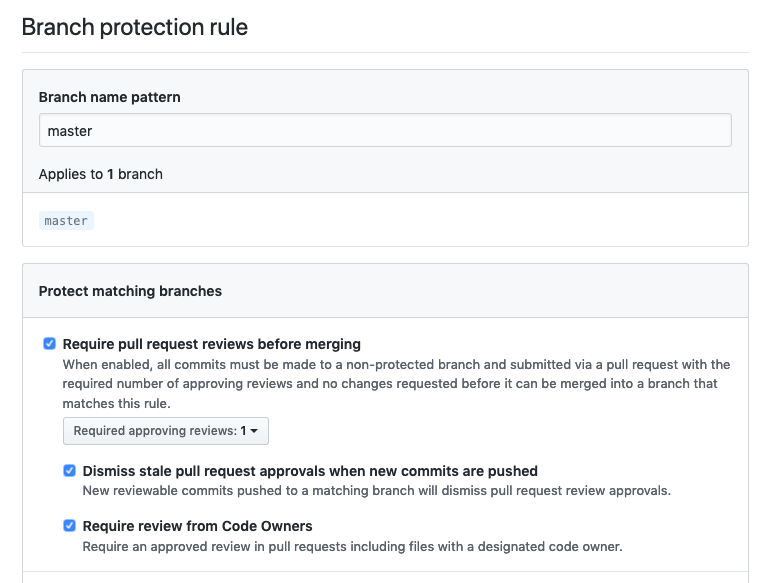
\includegraphics[scale=0.50]{images/github-branch-protection.png}
\caption{Setting up branch protection.}
\label{branchprotect}
\end{figure}

\justifying
After we start to work with CI/CD tools (status checks, like GitHub Actions for example) new choices, as seen in figure \ref{statuscheck}, become
available in this part of your repository for managing those checks.

\begin{figure}
\centering
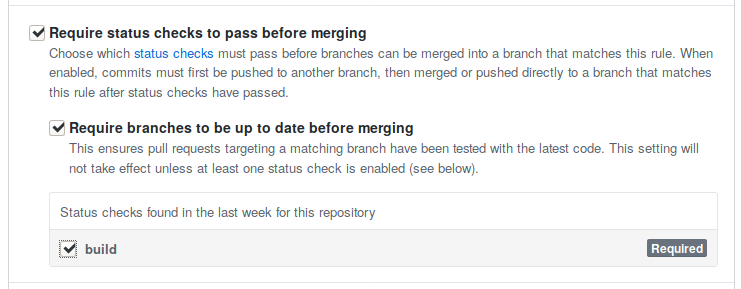
\includegraphics[scale=0.53]{images/guthub-status-check.png}
\caption{Requiring status checks.}
\label{statuscheck}
\end{figure}

\section{Branching and Merging}

When we say we are going to create a branch with git, it simply means we are going to take a snapshot of the code base at a point in time, and make our changes on that snapshot. The goal is to be able to make fixes and improvements without impacting the original code base.
Once our changes are completed, the typical process is to request a review from other team members and do some testing to make sure the changes will perform as expected. Once this is done, we are ready to merge our updated branch back into the main code base.

\subsection{Working with Branches}

\justifying
Naming your branches something useful is helpful (self documenting). Let's look at how to create a branch.

\subsection{Pull Requests}

\justifying
When you make changes on a local branch, say on your personal laptop, you will eventually want those changes
to flow back into the main project. Opening a pull request\index{Pull Request} is a means of letting other
people know you've got a set of changes ready for review and potential changes.

\justifying
Keeping pull requests smaller and more frequent makes it easier for your
peers to review your changes. It also means you will be less likely to lose work.

\subsection{Merging Your Branch}

\markdownInput{../labs/ch5/lab-5b.md}

\section{Forking and Cloning Existing Repositories}

\justifying
When someone else has a project on github.com that you would like to make changes to, you can make a ``fork'' of that project.
Forking\index{forking} a repository means you are making a copy of that repository to your personal account on the GitHub web
site. The reason for creating a fork is so we can make and test changes without any impact on the original repository.

\justifying
Once you have created a fork, you create a local copy of your fork on one or more of your personal workstations. This is
known as creating a ``clone'' \index{cloning a repo} of your fork. Now we have a workspace to make and test changes without
any impact to the parent repository. These changes or completed by creating one or more ``branches''. These branches and the
changes they encompass can be tested further, and are eventually merged into the parent repository.

\begin{figure}[!htb]
\centering
\input{dot/forking.tex}
\caption{Forking and cloning.}
\label{forkandclone}
\end{figure}

\justifying
This can be a tricky pattern to master, but it is fundamental if you
want to join the ranks of Open Source contributors and developers that
enjoy the full power of Git and GitHub.

\justifying
Adding a ``remote'' to your repository clone is a git convention to easily manage branches between your clone and
the original source repository.

\justifying
If you are starting out on a new project, simply creating a repo is probably enough. The whole fork/clone/merge to original
paradigm is better suited to medium to large size projects that accept contributions from multiple developers.

\markdownInput{../labs/ch5/lab-5c.md}

\section{Template Repositories}

\justifying
A GitHub Template Repository is available should you decide to follow along with the code examples in this book. The next sets of steps are
predicated on having Docker installed and running as described in the previous chapter.

\markdownInput{../labs/ch5/lab-5d.md}

\section{Conventions}

\subsection{CODEOWNERS}

\justifying
Creating a CODEOWNERS\index{CODEOWNERS} file is a good way to automatically tag folks in pull requests to make them aware of
changes to certain files or folders in your projects.

\justifying
In it's most basic form, the CODEOWNERS file in the .github directory simply lists the file(s) and the owner(s) on a line together.

\justifying
Consider this example where we add the ``@kevinflynn'' user to the CODEOWNERS file.

\begin{mybox}{\thetcbcounter: Adding a user to CODEOWNERS file}
      \lstinputlisting{code/22-github/create-codeowners.txt}
\end{mybox}

\justifying
In this example, the ``@kevinflynn'' user will be tagged as a reviewer in all pull requests.

\subsection{The .gitignore file}

\justifying
Use this file\index{.gitignore} to designate items that should be excluded from revision
control. This is useful for helping keep credentials and other secrets out of the GitHub repository.

\justifying
Consider the following example .gitignore file. This will prevent you from checking in the .DS-Store that
Macintosh creates in many folders.

\begin{mybox}{\thetcbcounter: Example .gitignore file}
      \lstinputlisting{code/22-github/create-gitignore.txt}
\end{mybox}

\section{Automated Repository Scanning}

\justifying
There are many GitHub plugins that are free for single-user/non-commercial scenarios. a cursory search of the web of the
GitHub Marketplace will turn up many of these. Let's leave some of the
tedious work to the bots, allowing us to focus on our DevSecOps journey to the cloud!

\justifying
\begin{tabular}{| p{2.3cm}| p{4.5cm} | p{8.5cm} |}
      \hline
     \textbf{Tool}& \textbf{Purpose}& \textbf{Source} \\
      \hline
      Renovate & dependency scanner & web site \\
      \hline
      lgtm & puppet-lint & Looks Good To Me \url{http://puppet-lint.com/} \\
      \hline
      metabob & AI based code review tool & website \\
      \hline
      bridgecrew & PR security scanner & web site \\
      \hline
\end{tabular}

\section{Directory Structure}

\justifying
Relevant files and folders mentioned in this chapter are organized as seen below.

\begin{figure}[!htb]
      \centering
      \input{dot/22-github.tex}
      \caption{GitHub related files.}
      \label{githubfiles}
\end{figure}

      \caption{GitHub related files.}
      \label{githubfiles}
\end{figure}

      \caption{GitHub related files.}
      \label{githubfiles}
\end{figure}

      \caption{GitHub related files.}
      \label{githubfiles}
\end{figure}
